\documentclass{../cours}
\usepackage{hyperref}
\title{Entraînement : listes chaînées}

\begin{document}
\maketitle

Les solutions peuvent être rédigées en \textbf{pseudo-code, python, C, C++ ou Java}. La syntaxe du langage n'a pas d'importance tant que celle-ci reste \textbf{cohérente} et \textbf{compréhensible}. (Dans les exemples, les solutions sont données en pseudo-code).

\textbf{Grille d'évaluation}

\vspace{0.5cm}

\begin{tabular}{|l|p{12cm}|}
\hline
A (20) & \small{L’algorithme répond au problème posé de façon claire et exhaustive.} \\ \hline
B (16) &\small{Le principe général de l'algorithme est le bon. Cependant, il y a une ou deux erreurs / oublis sur les cas particuliers ou les conditions d'arrêts et vérification de pointeurs nuls : ces erreurs impactent l'algorithme à la marge.} \\ \hline
C (11) & \small{Le principe général de l'algorithme est le bon mais les erreurs font que l'algorithme ne fonctionne pas dans de nombreux cas.}\\ \hline
D (8) &\small{Le principe général de l’algorithme ne permet pas de répondre au problème, cependant les opérations de manipulation sur la liste chaînée sont écrites correctement. Ou alors, même si le principe semble le bon, il y a de très nombreuses erreurs dans l'écriture.} \\ \hline
E (1) & \small{L’algorithme est faux ou inexistant et la structure de liste est mal utilisée.} \\ \hline
\end{tabular}


\begin{exercice}
Une \textbf{file} est une structure de données "First In, First out" : on fait sortir les éléments dans l'ordre dans lequel ils sont arrivés. Elle accepte deux opérations \textbf{enfile} qui rajoute un élément et \textbf{defile} qui supprime l'élément le plus ancien.

Exemple, si l'on part d'une file vide \texttt{F} :

\begin{lstlisting}
enfile(F,2)
enfile(F,1)
enfile(F,3)
enfile(F,4)
Affiche defile(F)
Affiche defile(F)
Affiche defile(F)
Affiche defile(F)
\end{lstlisting}

affiche $2134$.

Et 

\begin{lstlisting}
enfile(F,2)
enfile(F,1)
Affiche defile(F)
enfile(F,3)
enfile(F,4)
Affiche defile(F)
enfile(F,5)
Affiche defile(F)
Affiche defile(F)
Affiche defile(F)
\end{lstlisting}

affiche $21345$.

On propose d'implanter une File en utilisant une structure de liste chaînée. Cependant, contrairement à d'habitude, on va maintenir \textbf{deux pointeurs} : un sur la tête de liste et un sur le dernier élément de la liste. 

\begin{lstlisting}
Structure Cellule:
    Entier valeur
    Cellule suivante

Structure File:
    Cellule premiere
    Cellule derniere
\end{lstlisting}

On enfile en fin de liste et on défile en début de liste.

Exemple illustré.

\begin{tabular}{cccc}
Liste vide
&
Enfile 2
&
Enfile 4
&
Defile
\\
\scalebox{.8}{
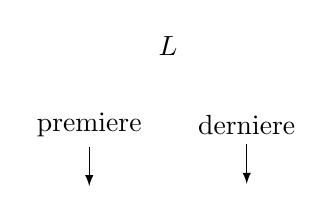
\begin{tikzpicture}[>=latex]
\node(L) at (1,0){$L$};
\node(Prem) at (0,-1){premiere};
\node(Dern) at (2,-1){derniere};

\draw (Prem.south) edge[->] ++(0,-.5);
\draw (Dern.south) edge[->] ++(0,-.5);
\end{tikzpicture}
}
&
\scalebox{.8}{
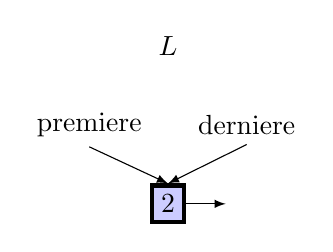
\begin{tikzpicture}[>=latex]
\node(L) at (1,0){$L$};
\node(Prem) at (0,-1){premiere};
\node(Dern) at (2,-1){derniere};

\node(T1)[draw, ultra thick, fill=blue!20, rectangle] at (1,-2) {2};

\draw (Prem.south) edge[->] (T1.north);
\draw (Dern.south) edge[->] (T1.north);
\draw (T1.east) edge[->] ++(.5,0);
\end{tikzpicture}
}
&
\scalebox{.8}{
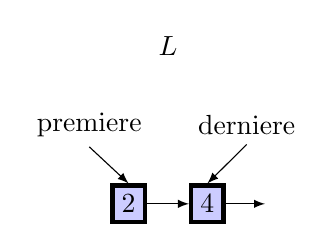
\begin{tikzpicture}[>=latex]
\node(L) at (1,0){$L$};
\node(Prem) at (0,-1){premiere};
\node(Dern) at (2,-1){derniere};

\node(T1)[draw, ultra thick, fill=blue!20, rectangle] at (0.5,-2) {2};
\node(T2)[draw, ultra thick, fill=blue!20, rectangle] at (1.5,-2) {4};

\draw (Prem.south) edge[->] (T1.north);
\draw (Dern.south) edge[->] (T2.north);
\draw (T1.east) edge[->] (T2.west);
\draw (T2.east) edge[->] ++(.5,0);
\end{tikzpicture}
}
&
\scalebox{.8}{
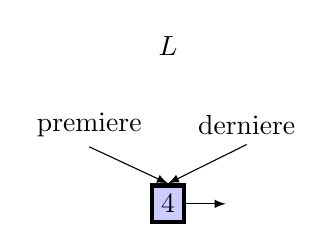
\begin{tikzpicture}[>=latex]
\node(L) at (1,0){$L$};
\node(Prem) at (0,-1){premiere};
\node(Dern) at (2,-1){derniere};

\node(T1)[draw, ultra thick, fill=blue!20, rectangle] at (1,-2) {4};

\draw (Prem.south) edge[->] (T1.north);
\draw (Dern.south) edge[->] (T1.north);
\draw (T1.east) edge[->] ++(.5,0);
\end{tikzpicture}
}
\\
\end{tabular}

Implantez les fonctions \texttt{Enfile(File F, Entier a)} (pas de valeur de retour) et \texttt{Defile(File F)} (renvoie un entier). On supposera
que l'appel \texttt{Cellule(a)} permet de créer une cellule de valeur $a$.


\textbf{Solution}

\begin{lstlisting}
Enfile
Input : File F, Entier a
Procédé :
    d <- F.derniere
    n <- Cellule(a) 
    Si d != None:
        d.suivante <- n
        F.derniere <- n
    Sinon:
        F.premiere <- n
        F.derniere <- n
        
Defile
Input : File F
Output : un entier
Procédé :
    p <- F.premiere
    Si p = None:
        Erreur
    Sinon
        v <- p.valeur
        F.premiere <- p.suivante
        Si F.premiere = None:
            F.derniere <- None
        Retourner v
\end{lstlisting}

\end{exercice}


\begin{exercice}[Partiel 2017-18]
On utilise la structure de donnée suivante :

\begin{lstlisting}
Structure Cellule:
    Entier valeur
    Cellule suivante

Structure Liste:
    Cellule premiere
\end{lstlisting}

Donner un algorithme qui prend en entrée une liste chaînée dont on suppose les valeurs ordonnées et qui supprime les occurrences multiples.

Par exemple, si la liste est 
\scalebox{.8}{
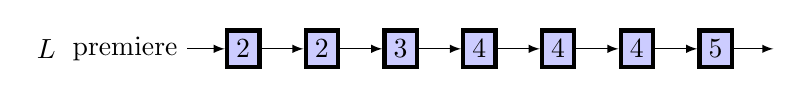
\begin{tikzpicture}[>=latex]
\node(L) at (-2,0){$L$};
\node(Prem) at (-1,0){premiere};

\node(T1)[draw, ultra thick, fill=blue!20, rectangle] at (0.5,0) {2};
\node(T2)[draw, ultra thick, fill=blue!20, rectangle] at (1.5,0) {2};
\node(T3)[draw, ultra thick, fill=blue!20, rectangle] at (2.5,0) {3};
\node(T4)[draw, ultra thick, fill=blue!20, rectangle] at (3.5,0) {4};
\node(T5)[draw, ultra thick, fill=blue!20, rectangle] at (4.5,0) {4};
\node(T6)[draw, ultra thick, fill=blue!20, rectangle] at (5.5,0) {4};
\node(T7)[draw, ultra thick, fill=blue!20, rectangle] at (6.5,0) {5};

\draw (Prem.east) edge[->] (T1.west);
\draw (T1.east) edge[->] (T2.west);
\draw (T2.east) edge[->] (T3.west);
\draw (T3.east) edge[->] (T4.west);
\draw (T4.east) edge[->] (T5.west);
\draw (T5.east) edge[->] (T6.west);
\draw (T6.east) edge[->] (T7.west);
\draw (T7.east) edge[->] ++(.5,0);
\end{tikzpicture}
}

Le résultat après le passage de l'algorithme sera
\scalebox{.8}{
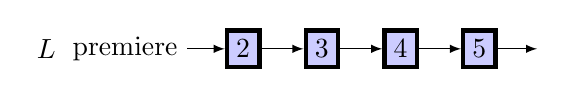
\begin{tikzpicture}[>=latex]
\node(L) at (-2,0){$L$};
\node(Prem) at (-1,0){premiere};

\node(T1)[draw, ultra thick, fill=blue!20, rectangle] at (0.5,0) {2};
\node(T2)[draw, ultra thick, fill=blue!20, rectangle] at (1.5,0) {3};
\node(T3)[draw, ultra thick, fill=blue!20, rectangle] at (2.5,0) {4};
\node(T4)[draw, ultra thick, fill=blue!20, rectangle] at (3.5,0) {5};

\draw (Prem.east) edge[->] (T1.west);
\draw (T1.east) edge[->] (T2.west);
\draw (T2.east) edge[->] (T3.west);
\draw (T3.east) edge[->] (T4.west);
\draw (T4.east) edge[->] ++(.5,0);
\end{tikzpicture}
}

\vspace{0.5cm}

\textbf{Solution}

Un algorithme possible (ce n'est pas le seul)

\begin{lstlisting}
Input : Une liste L
Procédé :
	c <- L.premiere
	Si c != None:
	   Tant que c.suivante != None:
	       v <- c.valeur
	       Si c.suivante.valeur == v:
	           c.suivante <- c.suivante.suivante
	       Sinon :
	           c <- c.suivante
\end{lstlisting}

Question donnée au partiel 1 2017-2018, résultats obtenus :

\begin{tabular}{|c|c|c|c|c|}
\hline
A & B & C & D & E \\ \hline
$28.6\%$ & $19\%$ & $42.9\%$ & $9.5\%$ & $0\%$ \\ \hline
\end{tabular} 

\vspace{0.5cm}

Exemple d'un algorithme qui obtient "B" :

\begin{lstlisting}
c <- L.premiere
Tant que c.suivante != None:
   v <- c.valeur
   Si c.suivante.valeur == v:
       c.suivante <- c.suivante.suivante
   Sinon :
       c <- c.suivante
\end{lstlisting}

Oubli de tester si \texttt{L.premiere} est \texttt{None} avant de faire \texttt{c.suivante} : l'algo ne fonctionne pas sur la liste vide.

Exemple d'un algorithme qui obtient "C" (le plus courant)

\begin{lstlisting}
c <- L.premiere
Si c != None:
   Tant que c.suivante != None:
       v <- c.valeur
       Si c.suivante.valeur == v:
           c.suivante <- c.suivante.suivante
       c <- c.suivante
\end{lstlisting}

On passe systématiquement à \texttt{c.suivante} : cet algorithme ne fonctionne pas dès qu'il y a plus de 2 copies d'une même cellule.

\end{exercice}


\begin{exercice}[Listes chaînées]
On utilise la structure de donnée suivante :

\begin{lstlisting}
Structure Cellule:
    Entier valeur
    Cellule suivante

Structure File:
    Cellule premiere
\end{lstlisting}

Donner un algorithme qui prend en entrée une liste chaînée et une valeur $a$ et qui supprime \textbf{toutes les occurences} de $a$ dans la liste.

Par exemple, si la liste est 
\scalebox{.8}{
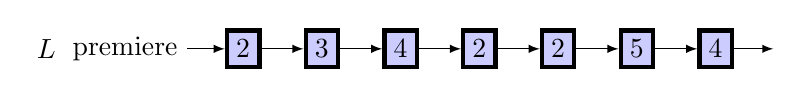
\begin{tikzpicture}[>=latex]
\node(L) at (-2,0){$L$};
\node(Prem) at (-1,0){premiere};

\node(T1)[draw, ultra thick, fill=blue!20, rectangle] at (0.5,0) {2};
\node(T2)[draw, ultra thick, fill=blue!20, rectangle] at (1.5,0) {3};
\node(T3)[draw, ultra thick, fill=blue!20, rectangle] at (2.5,0) {4};
\node(T4)[draw, ultra thick, fill=blue!20, rectangle] at (3.5,0) {2};
\node(T5)[draw, ultra thick, fill=blue!20, rectangle] at (4.5,0) {2};
\node(T6)[draw, ultra thick, fill=blue!20, rectangle] at (5.5,0) {5};
\node(T7)[draw, ultra thick, fill=blue!20, rectangle] at (6.5,0) {4};

\draw (Prem.east) edge[->] (T1.west);
\draw (T1.east) edge[->] (T2.west);
\draw (T2.east) edge[->] (T3.west);
\draw (T3.east) edge[->] (T4.west);
\draw (T4.east) edge[->] (T5.west);
\draw (T5.east) edge[->] (T6.west);
\draw (T6.east) edge[->] (T7.west);
\draw (T7.east) edge[->] ++(.5,0);
\end{tikzpicture}
}

Le résultat après le passage de l'algorithme supprimant $2$ sera
\scalebox{.8}{
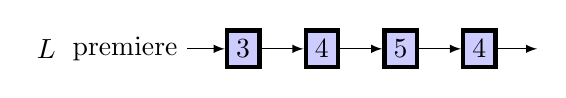
\begin{tikzpicture}[>=latex]
\node(L) at (-2,0){$L$};
\node(Prem) at (-1,0){premiere};

\node(T1)[draw, ultra thick, fill=blue!20, rectangle] at (0.5,0) {3};
\node(T2)[draw, ultra thick, fill=blue!20, rectangle] at (1.5,0) {4};
\node(T3)[draw, ultra thick, fill=blue!20, rectangle] at (2.5,0) {5};
\node(T4)[draw, ultra thick, fill=blue!20, rectangle] at (3.5,0) {4};

\draw (Prem.east) edge[->] (T1.west);
\draw (T1.east) edge[->] (T2.west);
\draw (T2.east) edge[->] (T3.west);
\draw (T3.east) edge[->] (T4.west);
\draw (T4.east) edge[->] ++(.5,0);
\end{tikzpicture}
}


\vspace{0.5cm}

\textbf{Solution}

Un algorithme possible (ce n'est pas le seul)

\begin{lstlisting}
Algo
Input : Liste L, valeur a
Procédé :
    c <- L.premiere
    Tant que c !=None et c.valeur == a:
        c <- c.suivante
    L.premiere <- c
    Tant que c != None:
        c2 <- c.suivante
        Tant que c2 != None et c2.valeur == a:
            c2 <- c2.suivante
        c.suivante <- c2
        c <- c.suivante

\end{lstlisting}

Question donnée au partiel 1 2018-2019, résultats obtenus :

\begin{tabular}{|c|c|c|c|c|}
\hline
A & B & C & D & E \\ \hline
$9\%$ & $41\%$ & $36\%$ & $13\%$ & $0\%$ \\ \hline
\end{tabular} 

\end{exercice}


\begin{exercice}[2019 -- 2020]
On utilise la structure de donnée suivante :

\begin{lstlisting}
Structure Cellule:
    Entier valeur
    Cellule suivante

Structure File:
    Cellule premiere
\end{lstlisting}

Donner un algorithme qui prend en entrée une liste chaînée et un entier $k$ et supprime les $k$ premiers éléments de la liste.

Par exemple, si la liste est 
\scalebox{.8}{
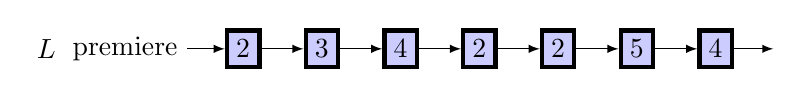
\begin{tikzpicture}[>=latex]
\node(L) at (-2,0){$L$};
\node(Prem) at (-1,0){premiere};

\node(T1)[draw, ultra thick, fill=blue!20, rectangle] at (0.5,0) {2};
\node(T2)[draw, ultra thick, fill=blue!20, rectangle] at (1.5,0) {3};
\node(T3)[draw, ultra thick, fill=blue!20, rectangle] at (2.5,0) {4};
\node(T4)[draw, ultra thick, fill=blue!20, rectangle] at (3.5,0) {2};
\node(T5)[draw, ultra thick, fill=blue!20, rectangle] at (4.5,0) {2};
\node(T6)[draw, ultra thick, fill=blue!20, rectangle] at (5.5,0) {5};
\node(T7)[draw, ultra thick, fill=blue!20, rectangle] at (6.5,0) {4};

\draw (Prem.east) edge[->] (T1.west);
\draw (T1.east) edge[->] (T2.west);
\draw (T2.east) edge[->] (T3.west);
\draw (T3.east) edge[->] (T4.west);
\draw (T4.east) edge[->] (T5.west);
\draw (T5.east) edge[->] (T6.west);
\draw (T6.east) edge[->] (T7.west);
\draw (T7.east) edge[->] ++(.5,0);
\end{tikzpicture}
}

Le résultat après le passage de l'algorithme avec $k=3$ sera 
\scalebox{.8}{
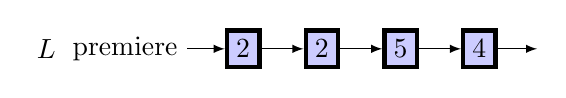
\begin{tikzpicture}[>=latex]
\node(L) at (1,0){$L$};
\node(Prem) at (2,0){premiere};

\node(T4)[draw, ultra thick, fill=blue!20, rectangle] at (3.5,0) {2};
\node(T5)[draw, ultra thick, fill=blue!20, rectangle] at (4.5,0) {2};
\node(T6)[draw, ultra thick, fill=blue!20, rectangle] at (5.5,0) {5};
\node(T7)[draw, ultra thick, fill=blue!20, rectangle] at (6.5,0) {4};

\draw (Prem.east) edge[->] (T4.west);

\draw (T4.east) edge[->] (T5.west);
\draw (T5.east) edge[->] (T6.west);
\draw (T6.east) edge[->] (T7.west);
\draw (T7.east) edge[->] ++(.5,0);
\end{tikzpicture}
}

\textbf{Solution}


\begin{lstlisting}
Algo
Input : Liste L, entier k
Procédé :
c <- L.premiere
i <- 0
Tant que i < k et c != None:
    i <- i+1
    c <- c.suivante
L.premiere <- c
\end{lstlisting}


Question donnée au partiel 1 2019-2020, résultats obtenus :

\begin{tabular}{|c|c|c|c|c|}
\hline
A & B & C & D & E \\ \hline
55\% & 30\% & 7\% & 4\% & 4\% \\ \hline
\end{tabular} 



\end{exercice}

\end{document}